\label{sec:special-case-gpmem}
We implement \gpmem\ by memoizing a target procedure in a wrapper that
remembers previously computed values.
This comes with interesting implications:
from the standpoint of computation, a data set of the form $\{(x_i,
y_i)\}$ can be thought of as a function $y = f_{\text{look-up}}(x)$,
where $f_{\text{look-up}}$ is restricted to only allow evaluation at a
specific set of inputs $x$.


Modelling the data set with a \ac{GP} then amounts to trying to learn
a smooth function $f_\emu$ (``emu'' stands for ``emulator'') which
extends $f$ to its full domain. We can then the incorporate
observations in two different ways: we can either constrain the
output of the emulator at a point \texttt{x} to a known value \texttt{y}:

    \begin{lstlisting}
    observe f_emu(x) = y
    \end{lstlisting}
or request a computation, which has the effect of constraining the
emulator to the copmuted value
    \begin{lstlisting}
    predict f_compute(x)
    \end{lstlisting}

The second expression has at least two benefits: (i) readability (in
some cases), and (ii) amenability to active learning.
As to (i), the statistical code of creating a Gaussian process is
replaced with a memoization-like idiom, which will be more familiar to
programmers.
As to (ii), when using \gpmem, it is quite easy to decide
incrementally which data point to sample next: for example, the loop
from \texttt{x[1]} to \texttt{x[n]} could be replaced by a loop in
which the next index \texttt{i} is chosen by a supplied decision rule.
In this way, we could use \gpmem\ to perform online learning using
only a subset of the available data.

We illustrate the use of \gpmem\ in this context in a tutorial in
Fig. \ref{fig:gpmem_tutorial}.

\begin{figure}
\centering
% for double arrows a la chef
% adapt line thickness and line width, if needed
\begin{tikzpicture}[thick]
\node[] (start) {};
 \node[draw,circle,minimum size=1.5cm,left = 0.5cm of start] (f) {f$_{\text{compute}}$};
 \node[draw,right = 0.5cm of start,circle,minimum size=1.5cm] (K) {$\mathbf{K}_{\theta}$};
 %\node[below left of=f_K,xshift=-1.7cm,yshift=-0.1cm] (theta) {$\bm{\theta} \sim P(\bm{\theta})$};
 \node[draw,rectangle,below=1.5cm of start, text width = 6.6cm] (gpmem) {\centering\texttt{gpmem}\vspace{2mm}
 
\small$\text{memo table} = (\mathbf{x}_{past},\mathbf{y}_{past})$\vspace{1.5mm}
 
 
\small$P(f_{emu}(x) \mid \mathbf{x}_{past},\mathbf{y}_{past})\sim \mathcal{N}(\mu(\mathbf{x}),\mathbf{K}_\theta\big(\mathbf{x},\mathbf{x})\big)$
 };
%  \node[draw,rectangle,color=ForestGreen,below = .1ex of gpmem,minimum width=1.5cm, minimum height=0.4cm,yshift=0.9cm,xshift=0.3cm] (mark) {};
  \node[draw,rectangle,dashed,right=2.2cm of K, text width = 2.2cm] (math) {\small
 $\mathbf{K}_{\theta} = \text{SE}(x,x^\prime)$\vspace{1.5mm}
 
 $\theta \;\;\,\,= \{sf,\ell \}$\vspace{1.5mm}
 
 $sf\;\, \sim P(sf)$\vspace{1.5mm}

 $\ell\;\;\;\; \sim P(\ell)$\vspace{1.5mm}
 
 
%\scriptnotesize
%
%%$\mu(\mathbf{x}) =\mu(\mathbf{x}) + \mathbf{K}_\theta(\mathbf{x},\mathbf{x}_{past})\mathbf{K}_\theta(\mathbf{x}_{past},\mathbf{x}_{past})^{-1}(\mathbf{y}_{past} - \mu(\mathbf{x}_{past}))$
 };
 \node[draw,rectangle,dashed,minimum size=1cm,left= 2.2cm of f] (resources) {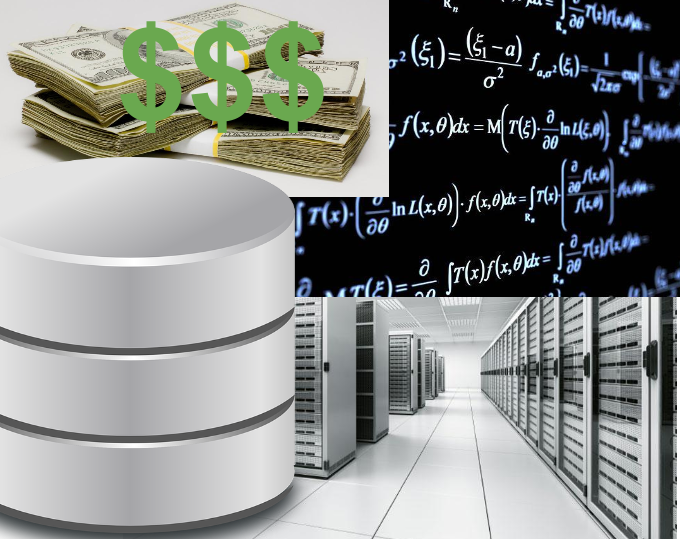
\includegraphics[width=3cm]{figs/resources.png}};

\node[draw,rectangle,below=1cm of gpmem,text width =7cm] (f_emu) {\centering $f_{emu}$ \vspace{2mm}

\begin{tabular}{l|l}\small
  $x$ & $f(x)$ \\ \hline
   $x_1$  & $y_1$ \\ 
   $x_2$  & $y_2$ \\
  $\cdots$ &   $\cdots$
 \end{tabular}
 $\;\;\;\;$
 \begin{tabular}{l}
 Parameters:\\
\small  Kernel lengthscale $\ell$  \\
\small Kernel scale-factor $sf$
 \end{tabular}

};
%\node[right = 1.2 cm of f_emu,inner sep = 0pt,outer sep=0pt,minimum size=25pt] (emu_annotate) {Infer: $\theta\;$};

\node[below = .1ex of gpmem,inner sep = 0pt,outer sep=0pt,xshift=-0.3cm] (helper1) {};
\node[below = .1ex of gpmem,inner sep = 0pt,outer sep=0pt,xshift=0.7cm] (helper2) {};

\node[above = .1ex of f_emu,inner sep = 0pt,outer sep=0pt, xshift=0mm] (helper_emu) {};

\node[above = 0.75cm of resources,inner sep = 0pt,outer sep=0pt] (helper_resource_top) {};
\node[left = 1cm of f_emu] (x_hat) {$\hat{x}$} ;
\node[right = 1cm of f_emu] (GaussianHat) {$\mathcal{N}(\hat{\bm\mu},\hat{\mathbf{K}})$} ;

%\node[right =1. cm  of f_emu, yshift=1.5cm] (infer) {\small Infer: $\ell$, $sf$} ;

% 1st pass: draw arrows

  \draw[thick,dashed,->] (resources) --node [pos=0.5,below] {resource}  node [pos=0.5,above] {outside} (f);
  \draw[thick,dashed,->] (math) -- node [pos=0.5,above] {Kernel} (K);
  \draw[thick,->] (K) -- (gpmem);
  \draw[thick,->] (f) -- (gpmem);
 % \draw[thick,->] (theta) -- (gpmem);
  \draw[thick,->] (gpmem) -- (f_emu);

 % \draw[thick,->,color=ForestGreen] (helper_compute) -- node[pos=0.5, sloped, below] {probe} (helper1);
 % \draw[thick,->,color=ForestGreen] (helper2) -- node[pos=0.5, sloped,above] {improves} (helper_emu);
   % \draw[thick,->,dashed,color=ForestGreen] (helper_resource) -- node[pos=0.5,above] {$f_{com}(x_2)=y_2$} (f_compute);
  %  \draw[thick,->,dashed,color=ForestGreen] (helper_resource) -- (resources);
     \draw[thick,->,dashed] (x_hat) -- (f_emu); 
     \draw[thick,->,dashed] (f_emu) -- (GaussianHat); 
 % \draw[thick,->] (theta) -- (gpmem);
  
   
%\path[](f_emu) edge [in=90, out=50,thick] (emu_annotate)
%    (emu_annotate) edge [->,in=310, out=270,thick]  (f_emu);
  % Note: If you have no branches, the 2nd pass is not needed

\end{tikzpicture}


\begin{tabular}{ll}
% line 1
& \\
\hline
\begin{lstlisting}[mathescape,escapechar=\#]
define f = proc( x) {
		    exp(-0.1*abs(x-2))) *
		    10* cos(0.4*x) + 0.2
		    }    
assume (f_compute f_emu) =  gpmem( f, K)
sample f_emu( array( -20, $\cdots$, 20)) 

\end{lstlisting}
& \raisebox{-0.5\height}{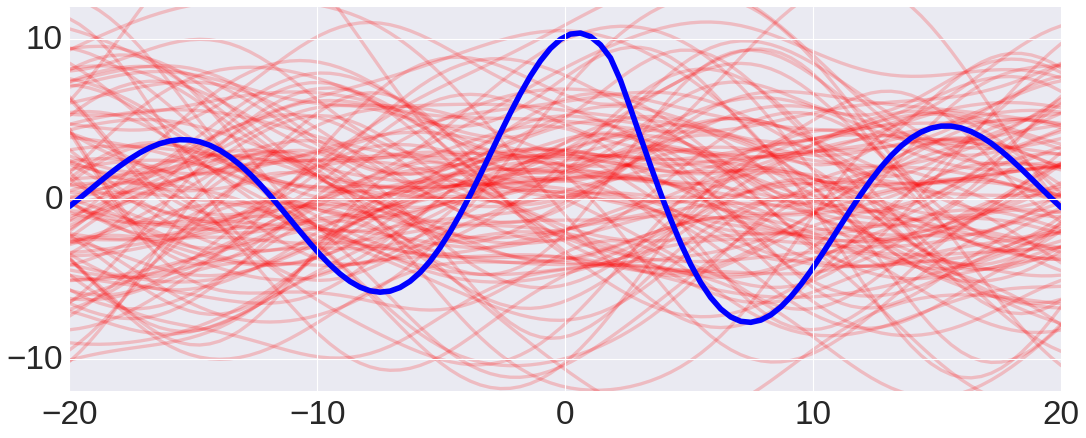
\includegraphics[height=2.5cm]{figs/tutorial_1.png}} \\ \hline
% line 2
\begin{lstlisting}[mathescape,escapechar=\#]
predict f_compute( 12.6)

sample f_emu( array( -20, $\cdots$, 20)) 

\end{lstlisting}
 &  \raisebox{-0.5\height}{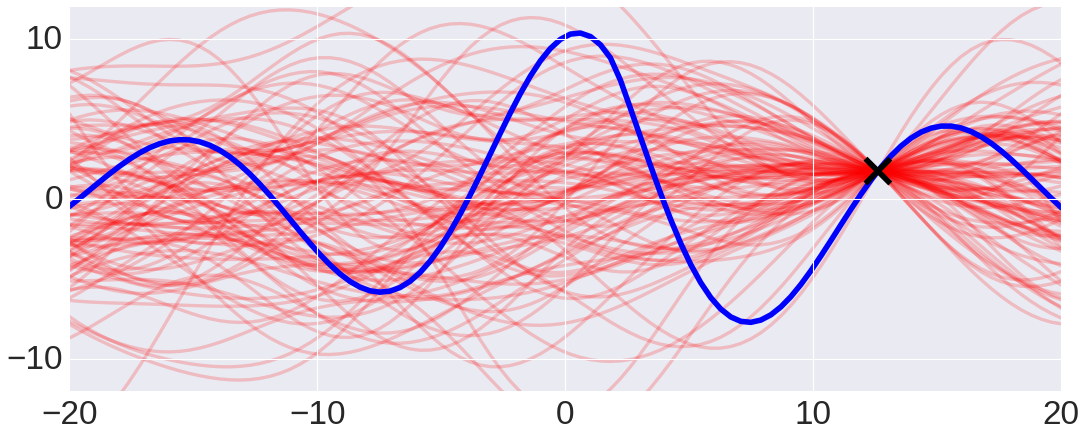
\includegraphics[height=2.5cm]{figs/tutorial_2.png}}  \\ \hline
% line 3 
 \begin{lstlisting}[mathescape,escapechar=\#]
predict f_compute( -6.4)

sample f_emu( array( -20, $\cdots$, 20)) 

\end{lstlisting}
 &  \raisebox{-0.5\height}{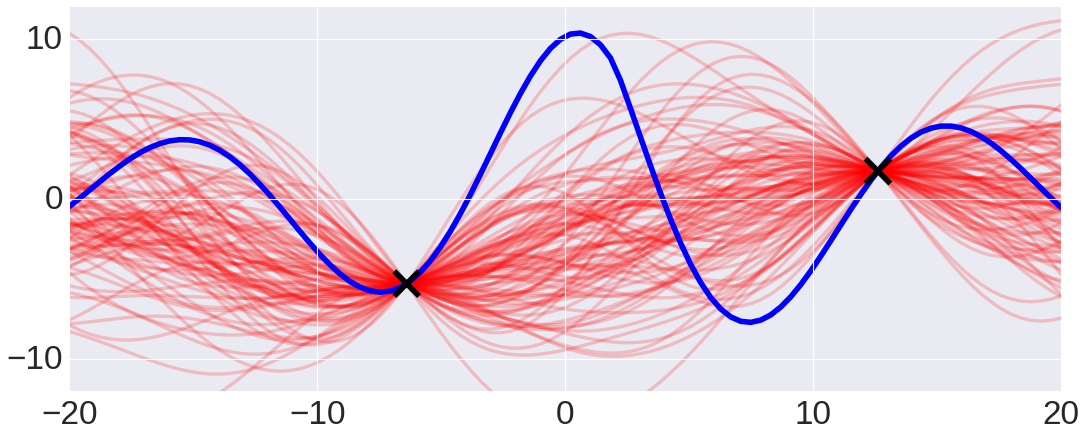
\includegraphics[height=2.5cm]{figs/tutorial_3.png}}  \\ \hline
% line 4
 \begin{lstlisting}[mathescape,escapechar=\#]
observe f_emu( -3.1) = 2.60 
observe f_emu( 7.8) = -7.60  
observe f_emu( 0.0) =  10.19

sample f_emu( array( -20, $\cdots$, 20)) 
  
\end{lstlisting}
 &   \raisebox{-0.5\height}{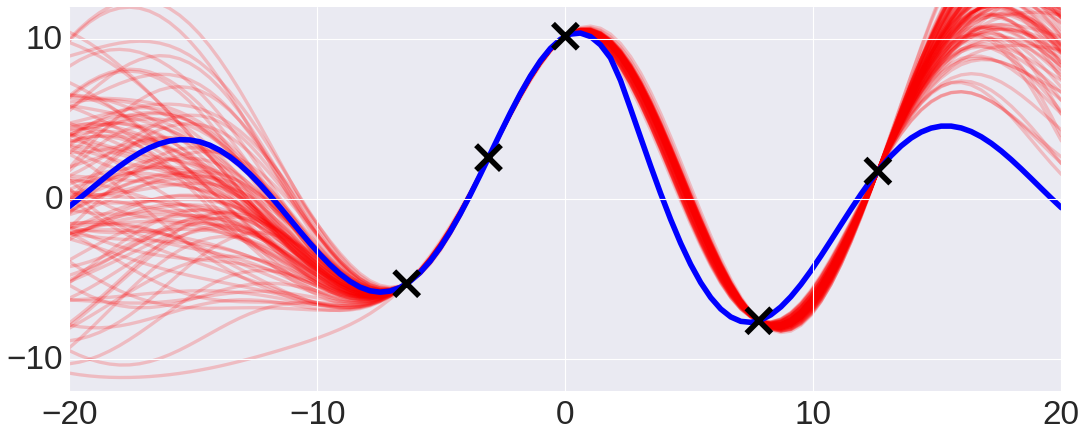
\includegraphics[height=2.5cm]{figs/tutorial_5.png}} \\ \hline
% line 5
 \begin{lstlisting}[mathescape,escapechar=\#]
infer mh(quote(hyper-parameter), one, 50)

sample f_emu( array( -20, $\cdots$, 20)) 
  
\end{lstlisting}
 &   \raisebox{-0.5\height}{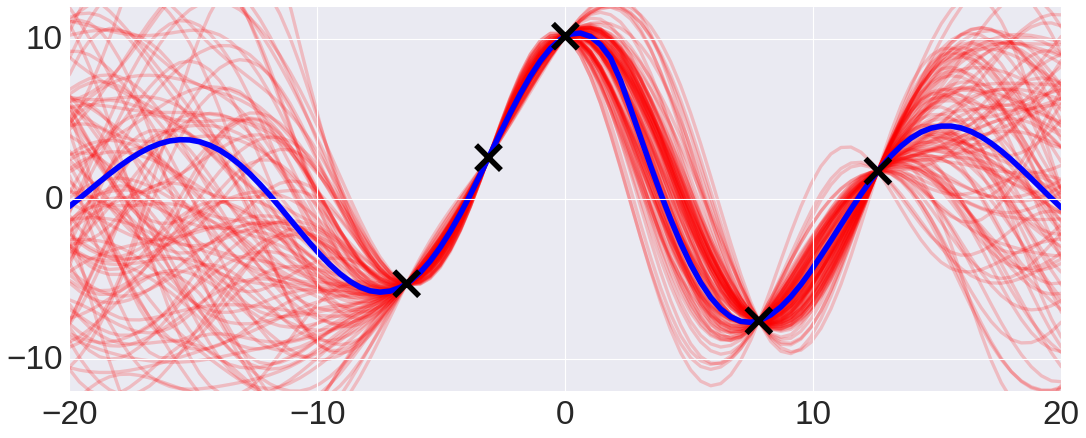
\includegraphics[height=2.5cm]{figs/tutorial_6.png}}
\end{tabular}
%\put(-245,10){\line(1,0){200}}
\put(-33,77){\color{ForestGreen}\thicklines \vector(0,-1){15}}
\put(-96,6){\color{ForestGreen}\thicklines \vector(0,-1){15}}
\put(-48,-63){\thicklines \vector(0,-1){15}}
\put(-84,-43){\thicklines \vector(0,-1){15}}
\put(-73,-68){\thicklines \vector(0,1){15}}
\caption{\gpmem\ tutorial. The top shows a schematic of \gpmem.
  \texttt{f\_compute} probes an outside resource.
  This can be expensive (top left).
  Every probe is memoized and improves the \ac{GP}-based
  emulator. Below the schematic we see a movie of the evolution
  of \gpmem's state of believe of the world given certain Venture
  directives.}
\label{fig:gpmem_tutorial}
\end{figure}
